\section{Antecedentes y trabajos relacionados} \label{sec:background}
En esta sección se comentan los principales conceptos necesarios para entender el resto del
documento, así mismo como un repaso a las técnicas que existen en la literatura para abordar
el problema tratado en este trabajo.\\
\subsection{Antecedentes}
Este trabajo se centra en la implementación, evaluación y mejora del algoritmo de predicción de
CI propuesto en \cite{2}. Para comprender mejor el contexto en el que se desarrolla,
primero vamos a presentar algunos de los conceptos básicos de CI y del problema que
nos ocupa. En primer lugar, se describirá el ciclo de vida de CI, junto a las dos
casuísticas que pueden darse en el proceso de integración. En segundo lugar, hablaremos sobre la
extracción de características, un aspecto fundamental para algoritmos de predicción. Por último,
se hablará del consumo de recursos computacionales que supone la implementación de CI,
de ahí la principal motivación de este trabajo, la reducción de dichos costes.


\subsubsection{El ciclo de vida de la Integración Continua.}
La Integración Continua es un proceso iterativo en el cual varios contribuidores hacen cambios
sobre un mismo código base añadiendo nuevas funcionalidades, para luego integrarlas a la misma
linea temporal de desarrollo, de forma controlada y automatizada. Cada integración se realiza
a través de la compilación, construcción y ejecución de pruebas automatizadas sobre el código
fuente \cite{10}. Aunque pueda parecerlo, la Integración Continua no es un proceso trivial, en
\cite{12} se describen las buenas prácticas de CI que deben seguirse para garantizar
la calidad del \textit{software}, algunas de las cuales han sido fuertemente adoptadas en el
sector, como por ejemplo:

\begin{enumerate}
      \item \textbf{Punto de código fuente único}: para faclitar la integración de cualquier
      desarrollador a un proyecto, es fundamental que este pueda obtener el código fuente
      actualizado del proyecto. La mejor práctica es utilizar un sistema de control de versiones
      como fuente única del código. Todos los archivos necesarios para la construcción del sistema,
      incluidos \textit{scripts} de instalación, archivos de configuración, etc., deben estar
      en el repositorio.
      \item \textbf{Automatización de \textit{builds}}: para proyectos pequeños, construir la
      aplicación puede ser tan sencillo como ejecutar un único comando. Sin embargo, para proyectos
      más complejos o con dependencias externas, la construcción puede ser un proceso complicado.
      El uso de \textit{scripts} de construcción automatizados es esencial para manejar estos
      procesos, llegando a analizar qué partes del código necesitan ser recompiladas, y gestionando
      dependencias para evitar recompilar innecesariamente.
      \item \textbf{Desarrollo de pruebas unitarias o de validación interna}: compilar el código
      no es suficiente para asegurar que funciona correctamente, por lo que se
      implementan pruebas automatizadas. Normalmente, estas se dividen en pruebas unitarias, que
      prueban partes específicas del código; y pruebas de aceptación, que prueban el sistema
      completo. Aunque este proceso no puede garantizar la ausencia total de errores, ofrece un
      mecanismo efectivo de mejorar la calidad del \textit{software} mediante la detección y
      corrección continua de fallos.
\end{enumerate}

Sin embargo, en el mundo real, la forma de aplicar cada una de estas técnicas y la prioridad con
la que se aplica puede estar fuertemente influenciada por la cultura empresarial donde
se desarrolle. En \cite{8}, se realiza un caso de estudio con tres empresas donde se percibe
que la adopción de las prácticas de CI no es homogénea. Por ejemplo, con respecto a tener
un único punto de código fuente, algunas prefieren minimizar los conflictos de fusión
(\textit{merge conflicts}) que el beneficio poco claro de usar un único repositorio. Por otro
lado, en cuanto a las pruebas unitarias, existen diferencias debido a limitaciones en las
herramientas (poco factibles para realizar pruebas de interfaz de usuario), a las percepciones
prácticas (el trabajo necesario para las pruebas de integración supera los beneficios percibidos)
y al contexto del proyecto (pruebas centradas en datos requieren comunicación con servicios
externos).\\

\textbf{Ejemplo práctico}: Un desarrollador hace un \textit{commit} (una
instantánea de los cambios realizados) y mediante una acción de \textit{push}, lo envía al
repositorio central. El servidor de CI \cite{9} (Jenkins, Travis CI, GitHub Actions,
etc.) detecta automáticamente este nuevo \textit{commit} y desencadena el \textit{pipeline} de
CI. El servidor extrae el nuevo código del repositorio y comienza a construir la
aplicación, lo que denominados la fase de construcción o \textit{build}. Esta parte puede incluir
la compilación del código fuente, la instalación de dependencias, etc. Una vez que la aplicación
está construida, se ejecutan una serie de pruebas automatizadas (\textit{Self-Testing code})
\cite{10}. Dichas pruebas pueden ser pruebas unitarias, pruebas de integración, pruebas
funcionales o pruebas de interfaz de usuario. Dependiendo del resultado de las fases anteriores,
podemos encontrarnos dos casos:

\begin{itemize}
    \item \textbf{La \textit{build} ha sido exitosa}: todas las pruebas han pasado con éxito. En
          este caso, el servidor de CI puede desplegar la aplicación en un entorno de
          pruebas o producción.\\
    \item \textbf{La \textit{build} ha fallado}: alguna de las pruebas ha fallado. En este caso,
          el servidor de CI suele notificar a los desarrolladores y detiene el
          despliegue de la aplicación.
\end{itemize}


\subsubsection{Características de las \textit{builds}.} \label{sec:features}
Al ejecutarse una \textit{build}, se pueden extraer de ella una serie de características con las
que algoritmos de predicción pueden predecir el resultado de la integración. Tener un conjunto
de \textit{features} bien seleccionadas y significativas mejorará la precisión de los modelos.
La mayoría de estudios utilizan catacteríticas extraídas directamente de la base de datos de
TravisTorrent \cite{6}, sin embargo, estas características no son las mejores para predecir
\textit{builds} que fallan, es decir, \textit{builds failures}. Algunos enfoques \cite{6,7}
hacen uso de características basadas en la \textit{build} actual, la \textit{build} anterior y
el histórico ligado a todas las ejecuciones de \textit{builds} anteriores. El primer estudio en
utilizar técnicas de \textit{Machine Learning} para predecir el resultado de CI fue realizado por
Hassan et al. \cite{7}. En su estudio, utilizó características basadas en la \textit{build} actual y la
anterior, para la \textit{build} anterior usó:

\begin{itemize}
      \item \textit{prev\_bl\_cluster}: el cluster de la \textit{build} anterior.
      \item \textit{prev\_tr\_status}: el estado de la \textit{build} anterior.
      \item \textit{prev\_gh\_src\_churn}: el número de líneas de código fuente cambiadas en la
            \textit{build} anterior.
      \item \textit{prev\_gh\_test\_churn}: el número de líneas de código de test cambiadas en la
            \textit{build} anterior.
\end{itemize}

Para la instancia de \textit{build} actual, se usaron características como:

\begin{itemize}
      \item \textit{gh\_team\_size}: el tamaño del equipo.
      \item \textit{cmt\_buildfilechangecount}: número de cambios en el archivo de script de
      construcción.
      \item \textit{gh\_other\_files}: número de archivos no relacionados con el código fuente.
      \item \textit{gh\_src\_churn}: número de líneas de código fuente cambiadas.
      \item \textit{gh\_src\_files}: número de archivos de código fuente.
      \item \textit{gh\_files\_modified}: número de archivos modificados.
      \item \textit{gh\_files\_deleted}: número de archivos eliminados.
      \item \textit{gh\_doc\_files}: número de archivos de documentación.
      \item \textit{cmt\_methodbodychangecount}: número de cambios en el cuerpo del método.
      \item \textit{cmt\_methodchangecount}: número de cambios en la cabecera del método.
      \item \textit{cmt\_importchangecount}: número de cambios en los \textit{imports}.
      \item \textit{cmt\_fieldchangecount}: número de cambios en los atributos de clase.
      \item \textit{day\_of\_week}: día de la semana del primer \textit{commit} de la
      \textit{build}.
      \item \textit{cmt\_classchangecount}: número de clases cambiadas.
      \item \textit{gh\_files\_added}: número de archivos añadidos.
      \item \textit{gh\_test\_churn}: número de líneas de código de test cambiadas.
\end{itemize}

En \cite{6} se reutilizaron gran cantidad de estas features mencionadas añadiendo las
relacionadas con el histórico de ejecuciones de \textit{builds}: tanto por ciento de compilaciones
fallidas, incremento del \textit{fail} ratio en la última \textit{build} con respecto al ratio
de la penúltima, porcentaje de \textit{builds} exitosas desde la última \textit{build} fallida,
etc. Como vemos, se utilizan un gran número de \textit{features} para la predicción, sin embargo,
el objetivo no es la reducción de los costos de CI ni la  importancia de cada una de
ellas en relación con los \textit{build failures}. El hecho de que se utilicen tantas
\textit{features} relacionadas con la \textit{build} anterior, hace que predecir una
\textit{build} como fallida esté fuertemente relacionado con el resultado de la \textit{build}
anterior, que debería ser fallida. Esto hace que exista una limitación para la detección de los
primeros \textit{build failures} \cite{2}, ya que estos dependen mucho del resultado de la
\textit{build} anterior y, por definición, estarán siempre precedidos por una \textit{build}
exitosa.\\

Los \textit{build failures} pueden categorizarse en una serie de tipos. Se ha identificado un
total de 14 categorías de build failures, clasificadas según el tipo de error que las origina
\cite{13}. En el estudio se demostró que más
del 80\% de los errores se producían en la fase de ejecución de pruebas o \textit{tests}. En
el estudio se pretende identificar las causas que originan los \textit{build failures}, para lo
que se usan $16$ métricas de la literatura y se descubre lo siguiente:

\begin{itemize}
      \item Se respalda la hipótesis de que los \textit{build failures} pueden aumentar con la 
      complejidad de los cambios.
      \item Cambios objetivamente insignificantes pueden romper la \textit{build}.
      \item Hay poca evidencia de que la fecha y hora de un cambio tenga un aspecto negativo o
      positivo en los resultados.
      \item Los autores que \textit{commitean} menos frecuentemente tienden a causar menos
      \textit{build failures}.
      \item Normalmente, las \textit{builds} lanzadas a través de \textit{pull requests} fallan
      con mayor frecuencia que las lanzadas por cambios directamente subidos a través de
      \textit{push} a la rama principal.
      \item No existe evidencia que demuestre que trabajar en paralelo a un \textit{pull request}
      afecte al resultado de la \textit{build}.
      \item La mayoría de los errores se producen consecutivamente. Las fases más inestables de
      compilación generan fallos en la CI.
\end{itemize}

Todos estos resultados se obtuvieron a través de un estudio empírico con 14 proyectos de código
abierto basados en Java que usan Travis CI. Por último, en \cite{16} se realiza un estudio a gran
escala con 3.6 millones de \textit{builds} en el que se demuestra que factores como la cantidad
de cambios en el código fuente, el número de \textit{commits}, el número de archivos modificados
o la herramienta de integración usada tienen una relación estadísticamente significativa con las
compilaciones fallidas.\\ 

\subsubsection{El costo de la Integración Continua.}
La implementación de la Integración Continua, a pesar de ofrecer numerosas ventajas, también
supone un coste computacional y económico. Además del costo computacional que supone ejecutar
la CI, debemos sumarle el costo del tiempo no productivo de los desarrolladores si estos
no saben como proceder sin saber el resultado de la integración. Hilton et al. \cite{10} estudiaron
los beneficios y costes de aplicar CI en proyectos de código abierto. En su estudio,
observaron que entre los proyectos \textit{open-source} que no usaban CI, el principal
motivo no era el costo técnico, si no que los desarrolladores no estaban familiarizados con
CI. Otra de las razones de no usar CI era la falta de \textit{tests} automáticos,
un aspecto fundamental en CI. Además, calcularon el costo de mantenimiento de la
CI, para lo que midieron el número de cambios en los archivos de configuración. Observaron
que el número medio de modificaciones en archivos de configuración se elevaba a 12, siendo
frecuente que se realizaran cambios en la configuración de CI. Una de las principales
razones para estos cambios en archivos de configuración era la presencia de versiones obsoletas
en las dependencias. Por último, observaron un hecho curioso con respecto al tiempo de ejecución
medio de las \textit{builds}: las \textit{builds} exitosas son, en promedio, más rápidas que
aquellas que fallan. Intuitivamente, podría esperarse lo contrario, ya que un error debería de
interrumpir el proceso antes, aunque se necesita una mayor investigación para averiguar estas
razones.\\

Klotins et al. \cite{18} realizaron un trabajo con múltiples casos de estudio en el que
encontraron que la aplicación de CI mejoraba notablemente los procesos de desarrollo
internos en las empresas, sin embargo, se destaca la necesidad de evaluar las consecuencias de
aplicar este tipo de desarrollo desde una perspectiva del cliente. El hecho de actualizar a los
clientes a entregas continuas es un obstáculo importante ya que pueden existir acuerdos previos,
y renegociar dichos acuerdos conlleva el riesgo de perder clientes y causar inestabilidad en la
empresa. En el estudio se ha observado la necesidad de adoptar prácticas de CI para
mejorar los procesos de desarrollo \textit{software} en las empresas, sin embargo, estas se
enfrentan a desafíos comunes en su implementación:

\begin{enumerate}
	\item \textbf{Beneficios internos vs. externos}: se reconocen los beneficios internos de
      aplicar CI, como la agilización de los procesos y la liberación de recursos. Sin
      embargo, extender estos beneficios a los clientes y la adaptación de los modelos de negocio
      existentes representan un obstáculo mayor.
	\item \textbf{Cultura organizacional}: la implementación de CI requiere cambios
      significativos en los procesos y en la cultura organizacional. Esto requiere compromiso por
      parte de los equipos de desarrollo y directivos.
	\item \textbf{Clientes}: convencer a los clientes para aceptar entregas más frecuentes y
      compartir más datos es fundamental para sacar partido a las ventajas de CI. Sin
      embargo, los clientes pueden ofrecer resistencia al cambio y esto puede poner en peligro
      las relaciones con los mismos.
\end{enumerate}

En \cite{17} se presenta un estudio en el que se preguntó a trabajadores de la empresa
\textit{Atlassian} sobre sus percepciones sobre los fallos de CI. Entre los trabajadores,
una gran mayoría (46\%) consideraba como muy o extremadamente difícil resolver los fallos de
CI, una minoría (13\%) consideraba que no era difícil resolverlos, y el resto calificó
la complejidad como moderada. Además, comentaban que los fallos de CI podían afectar tanto
al flujo de trabajo individual como a la empresa. Los trabajadores notaban que estos fallos podían
aumentar el tiempo de trabajo e incluso interrumpir el flujo de desarrollo. Otro impacto posible
es la reducción de la productividad, ya que alguien tiene que dedicar tiempo a investigar por qué
falló la \textit{build} y solucionarlo. Este tipo de problemas puede ocasionar que las revisiones
o las correcciones rápidas tarden más tiempo de lo esperado, poniendo en peligro el tiempo de
lanzamiento (\textit{release}). Además, se menciona que factores técnicos como humanos desempeñan
un papel fundamental en la adopción de CI.\\

\subsection{Trabajos relacionados} \label{sec:related_work}
Existen numerosos estudios que buscan reducir el costo asociado a la Integración Continua
mediante la creación de \textit{predictors} \cite{7,5,2,15,6,14,4,1,19}. Hassan et al. \cite{7}
estudiaron un total de 402 proyectos Java con información de 256,055 \textit{builds}, procedentes
de la base de datos de TravisTorrent. En su estudio se utilizan características extraídas
directamente de la base de datos de TravisTorrent y otras propias, relacionando \textit{features}
propias de la \textit{build actual} y la anterior. En su propuesta, primero se realiza una
selección de \textit{features} basada en la evaluación de la importancia de las mismas mediante
el \textit{Information Gain (IG)}. Con ello seleccionan las más discriminativas del conjunto de
\textit{features} (Sección \ref{sec:features}). Posteriormente, construyen un clasificador que usa
\textit{random forest} para clasificar las \textit{builds} en exitosas y fallidas. Este estudio
fue el primer enfoque en utilizar técnicas de \textit{Machine Learning} para predecir el resultado
de la CI, sin embargo, no estaba centrado en reducir los costos asociados a la misma ni
a los \textit{build failures}, los casos positivos que más interés tienen.\\

En \cite{5} se propone una solución novedosa que usa Programación Genética Multi-Objetivo, sin
utilizar técnicas de aprendizaje automático. Su enfoque consiste en recopilar \textit{builds}
exitosas y fallidas de un proyecto, obtener información de \textit{TravisTorrent} que contiene
información sobre \textit{builds} de \textit{Travis CI} y, a partir de ahí, se toman esos datos
como entrada para generar un conjunto de reglas predictivas que anticipen el resultado de la
compilación de CI con la mayor precisión posible. Finalmente, entra en juego el 
algoritmo de programación genética multiobjetivo, el cual va generando un conjunto de soluciones, 
cada una de ellas con su conjunto de reglas de predicción, por ejemplo, una combinación de
umbrales asignados a cada métrica. Dicha combinación de métricas-umbrales está conectada a
operadores lógicos. Todas las muestras generadas en la solución son evaluadas usando dos
objetivos: maximizar la tasa de verdaderos positivos y, minimizar la tasa de falsos positivos.
En cada iteración se van cambiando los operadores, generando nuevas soluciones, hasta llegar a
una condición de parada y devolviendo la solución óptima. En el estudio encontraron que
características como el tamaño del equipo, la información de la última \textit{build} o el tipo
de archivos cambiados, pueden indicar el potencial fallo de una \textit{build}. A pesar de
obtener buenos resultados, solo se centran en 10 proyectos de lenguajes Java y Ruby, haciendo
poco generalizables sus resultados. Además, el ratio de \textit{failures} que presentan estos
proyectos es relativamente elevado, lo que puede ocasionar que el algoritmo no sea tan efectivo
en proyectos con ratios de \textit{failures} bajos.\\

La piedra angular de nuestro estudio se basa en el trabajo de \textbf{Servant et al.} \cite{2}. En
este estudio, se propone un algoritmo que utiliza técnicas de \textit{Machine Learning}
para la predicción de CI, con el objetivo de reducir los costos asociados a la misma.
Su teoría parte de dos hipótesis principales:

\begin{itemize}
      \item \textit{$H_1$}: la mayoría de las \textit{builds} devuelven un resultado exitoso. Por
      lo general, las \textit{builds} exitosas son más numerosas que las fallidas. Es decir,
      siempre habrá mayor ratio de \textit{builds} que pasan la CI que \textit{builds}
      que fallan.
      \item \textit{$H_2$}: muchas \textit{builds} fallidas en CI ocurren
      consecutivamente después de otra \textit{build} fallida.
\end{itemize}

Teniendo en cuenta estas dos hipótesis encontramos que, si la primera es cierta, al saltarse todas
aquellas \textit{builds} que se predigan como exitosas, se reducirá el coste considerablemente.
En caso de que la segunda sea cierta, entonces si se predice que las \textit{builds} subsecuentes a una
\textit{build} fallida también fallarán, se predecirán correctamente una buena parte de las
\textit{builds} fallidas. En el estudio se introduce por primera vez el término de \textit{first
failures}, que hace referencia a las primeras \textit{builds} que fallan en una subsecuencia de
\textit{builds failures}. En enfoques anteriores, existe una limitación para la predicción
de estas primeras \textit{builds} que fallan, ya que dependen fuertemente del resultado de la
\textit{build} anterior, haciendo que sean complicadas de predecir.\\

En el algoritmo, se utilizan \textit{features} que son propias de la \textit{build} y
sirven para predecir \textit{build failures} en un mismo proyecto y, por otro lado, se usan
\textit{project features}, que sirven para realizar lo que se denomina \textit{cross-project
predictions}. Con respecto a las \textit{build features}, estas son propias de la \textit{build}
en cuestión y servirán para realizar predicciones sobre el mismo repositorio que estemos
analizando. En el estudio, se mencionan algunas más, pero finalmente se seleccionan las
siguientes:

\begin{itemize}
      \item \textbf{SC}: el número de líneas de código fuente cambiadas desde la
      última \textit{build}.
      \item \textbf{FC}: el número de archivos modificados desde la última
      \textit{build}.
      \item \textbf{TC}: el número de lineas de \textit{tests} cambiadas desde la
      última \textit{build}.
      \item \textbf{NC}: el número de \textit{commits} desde la última \textit{build}.
\end{itemize}

En cuanto a las \textit{project features}, estas son útiles cuando queremos predecir
el resultado de la CI en un proyecto que tiene un número escaso de \textit{builds}, bien
porque sea reciente, no se hayan ejecutado en su duración gran número de \textit{builds}, etc. Este
último problema es lo que suele denominarse en sistemas de información como el ``arranque en frío''
(\textit{cold start}), cuando no se puede extraer información útil para los usuarios debido a
que todavía no se ha reunido suficiente información. Para ello, se usan modelos generados a partir
de otros proyectos entrenados con estas \textit{features}. En el estudio, se mencionan algunas
\textit{project features}, pero finalmente se seleccionan las siguientes:

\begin{itemize}
      \item \textbf{TD}: el número medio de líneas en los casos de prueba por cada
      1000 líneas ejecutables de código de producción.
      \item \textbf{PS}: el número medio de líneas de código fuente de producción
      ejecutale en el repositorio a lo largo de la historia de uso de CI en el proyecto.
      \item \textbf{PA}: la duración entre la primera y la última \textit{build} del
      proyecto
\end{itemize}


\noindent A continuación, se explica de forma gráfica el funcionamiento de su algoritmo, llamado
SmartBuildSkip:

\begin{figure}[H]
      \centering
      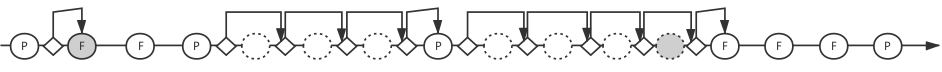
\includegraphics[scale=0.49]{images/SBS.png}
      \caption{Línea temporal de SmartBuildSkip \cite{2}.}
      \label{fig:timeline SBS}
\end{figure}

Cada círculo recoge el resultado real de la \textit{build}. Los \textit{first failures} están
sombreados en gris. El símbolo de diamante indica que el predictor ha realizado una predicción.
Las \textit{builds} que se han saltado están indicadas con círculos discontinuos. Cuando una
\textit{build} se predice como \textit{pass}, el algoritmo acumula los cambios de la
\textit{build} con la siguiente, lo que se indica mediante una flecha entre los círculos. Cuando
se predice un \textit{first failure}, \textit{SmartBuildSkip} predice directamente como
\textit{fail} la \textit{build} siguiente. Así, hasta que se encuentra un \textit{pass}, lo que
vuelve a reiniciar el algoritmo a la primera fase de predicción.\\

Se ha elegido este estudio \cite{2} como base para nuestro trabajo porque es el primero que usa
únicamente \textit{features} que presentan una correlación significativa con las \textit{build
failures}. Además, con nuestro trabajo pretendemos indagar en la calidad de estas \textit{features}
y en mejorar los resultados obtenidos en el estudio original, bien mediante la adición de nuevas
\textit{features} o mediante la mejora del algoritmo de predicción.\\

Continuando con el orden cronológico del estado del arte, Saidani et al. \cite{15} propone un
predictor que utiliza Redes Neuronales Recurrentes (RNN) basadas en Memoria a Largo
Plazo (LSTM). Su estudio se realiza como es habitual con diez proyectos de código
abierto que usan el sistema de CI de \textit{Travis CI}, sumando un total de 91330
\textit{builds}. Estos revelan que este tipo de técnicas ofrecen mejores resultados
que las de \textit{Machine Learning}, obteniendo mejor rendimiento en términos de AUC,
\textit{F1-Score} y \textit{accuracy} cuando se trata de validación entre proyectos. En \cite{6}
se propone una nueva solución en la que se usa un predictor que es dependiente del histórico de
\textit{builds} pasadas para poder hacer sus predicciones. En este estudio existen métodos de
selección de \textit{features} que selecionan determinadas \textit{features} en función del tipo
de proyecto que se esté evaluando. En otro artículo, Ouni et al. \cite{14} propone una solución
de línea de comandos donde se consigue mejorar el estado del arte en términos de \textit{F1-Score}.
Sin embargo, en el estudio, solo se tiene en cuenta el estudio \cite{7} comentado anteriormente,
obviando todas las implementaciones posteriores y teniendo una clara amenaza a la validez del
mismo. Además, dada la arquitectura presentada, podemos apreciar que para la extracción de
\textit{features}, se utiliza un parseador de HTML con \textit{Jsoup} y \textit{Selenium},
lo cuál hace poco duradero el enfoque, ya que está fuertemente acoplado a la estructura
HTML de \textit{GitHub} y sus cambios. \\

Jin et al. \cite{4} propone un nuevo predictor, \textit{PreciseBuildSkip}, que mejora el ahorro
de costo y la observación de \textit{builds} fallidas, llegando a obtener valores de
\textit{recall} realmente buenos. En su implementación, incluyen dos variantes: la segura, que
salva el 5.5\% de las \textit{builds} y por lo general captura todas las construcciones fallidas,
y una versión que mejora el ahorro de costos, salvando un 35\% de las \textit{builds} mientras
captura un 81\% de las observaciones de \textit{builds} fallidas. Finalmente, Jin et al. \cite{1} propone
una solución que emplea técnicas de selección de \textit{builds} y dos técnicas de selección de
tests. Esta solución ejecuta seis técnicas existentes y luego usa los resultados como
\textit{features} para un clasificador \textit{Random forest}. Entre sus resultados, se observa
que:

\begin{itemize}
      \item Se consiguió un mayor ahorro de costos con la mayor seguridad en comparación con
      técnicas anteriores.
      \item Tener un componente de selección de \textit{tests} además de un componente de
      selección de compilación aumenta los ahorros de costos.
      \item Tener enfoques de selección de \textit{tests} para predecir los resultados aumenta
      tanto la capacidad de ahorro de costos como la capacidad de observación de \textit{build
      failures}.
      \item El algoritmo de bosque aleatorio es el que ofrece mejor rendimiento en la predicción.
      \item La \textit{features} que recoge los fallos consecutivos fue la más efectiva para este
      enfoque.
\end{itemize}

Por otro lado, no existen proyectos documentados que usen técnicas de predicción de CI
para el ahorro de costos, por lo que es complicado evaluar el impacto económico real que estas
pueden causar. Liu et al. \cite{19} utiliza simulación de procesos \textit{software} y
experimentos basados en simulación para evaluar el impacto de estos \textit{predictors} de
CI en un entorno más realista. Entre sus descubrimientos, vieron que existe poca
diferencia entre los \textit{predictors} del esado del arte y las estrategias aleatorias en
términos de ahorro de tiempo. Sin embargo, en casos donde el ratio de \textit{builds} fallidas
es mayor, la estrategia aleatoria tendría un impacto negativo. Además, en proyectos donde la
proporción de \textit{failures} es muy pequeña, el uso de CI predictiva no es mucho
mejor que saltar \textit{builds} de forma aleatoria. A pesar de esto, se demuestra que el uso
de técnicas de \textit{predictive CI} puede ayudar a ahorrar el costo de tiempo para ejecutar
CI, así como el tiempo promedio de espera antes de ejecutar la CI.
